\chapter{Экспериментальное исследование параметров устройства квантовой коммуникации с недоверенным приемным узлом} \label{ch:ch5}
\section{Интерференция сигналов на боковых частотах фазомодулированного излучения} \label{sec:ch5/sec1}


 \begin{figure}[ht]
  \centering
  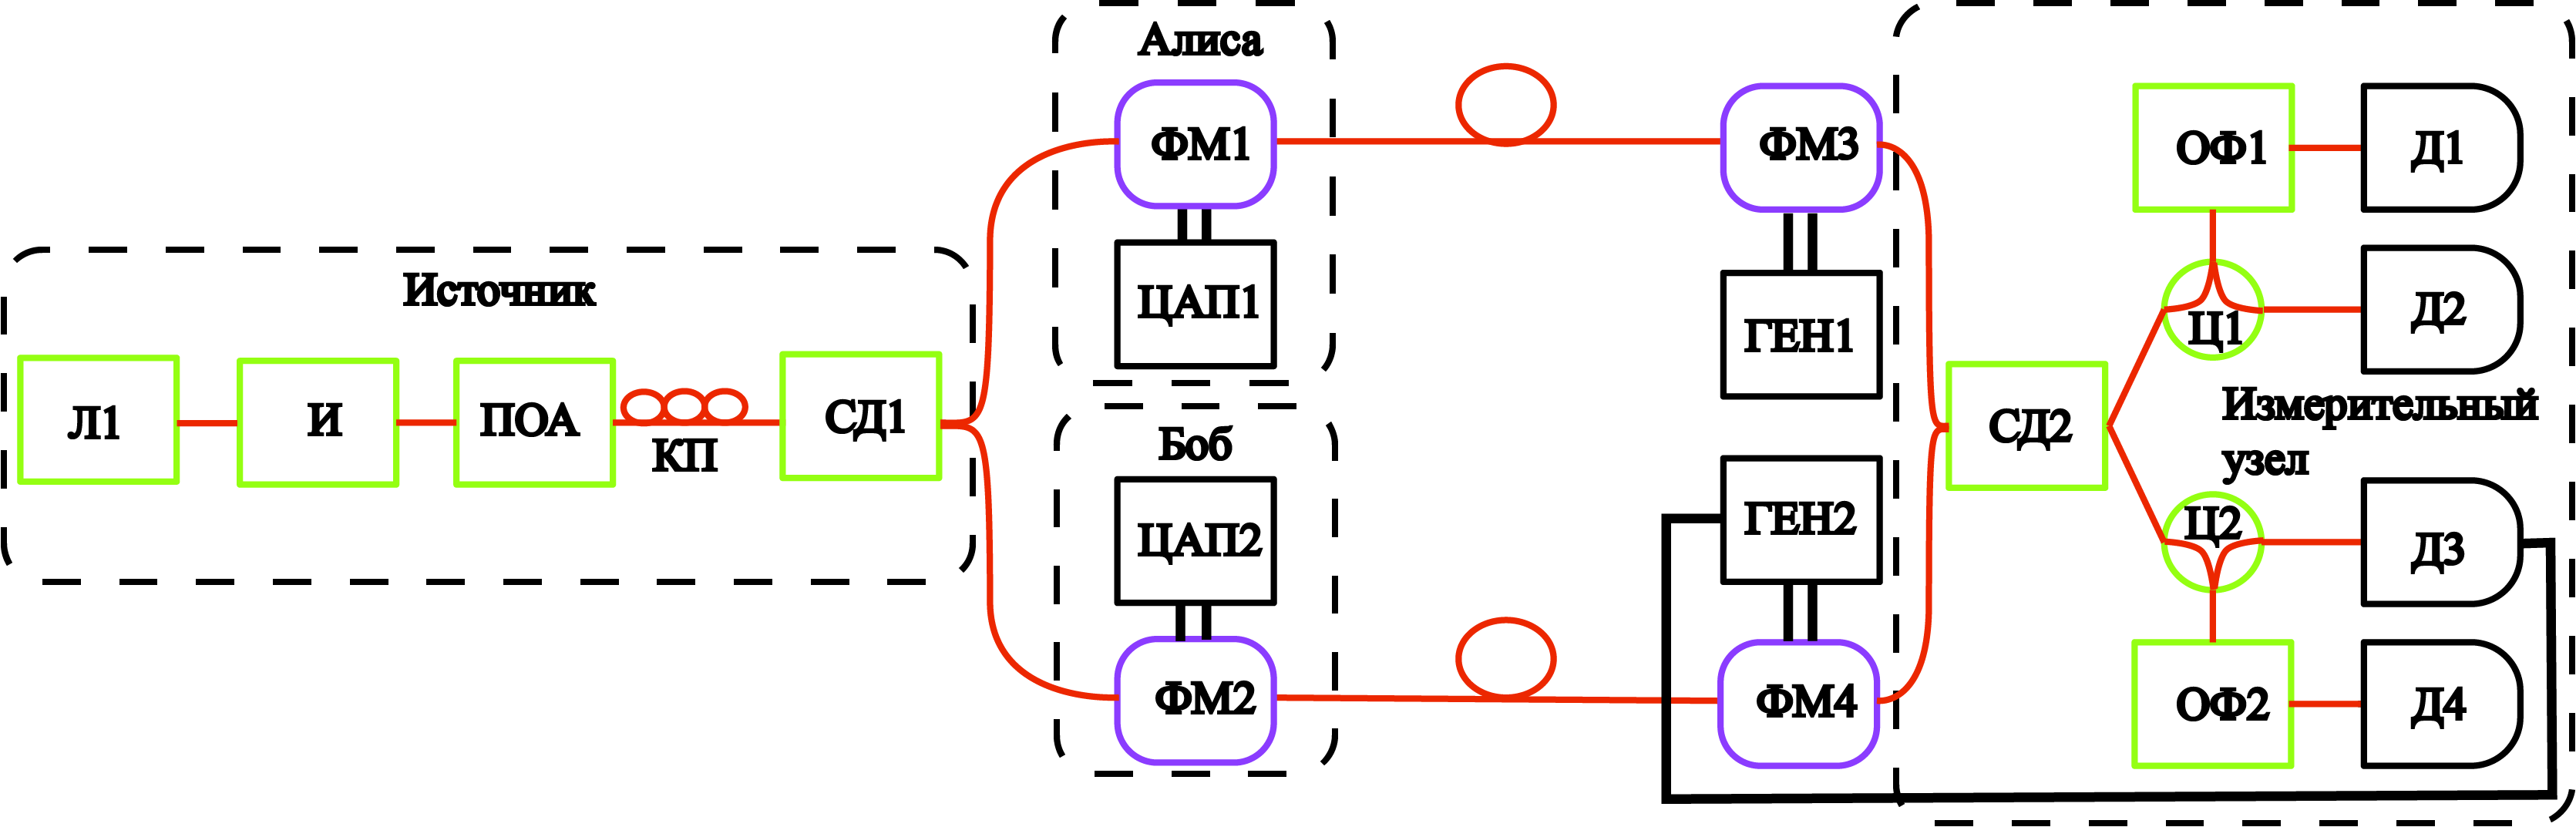
\includegraphics[scale=0.5]{Scheme_colored_rus.png}
  \caption{Принципиальная схема экспериментального стенда}
  \label{fig:RF_sin}
\end{figure}

\pagebreak

%%%%%%%%%%%%%%%%%%%%%%%%%%%%%%%%%%%%%%%%%%%%%%%%%%%%%%%%%%%%%%%%%%%%%%%%%%%%%%%%%
\section{Характеристики компонентов экспериментального стенда} \label{ch:ch5/sect2}

 \begin{figure}[ht]
  \centering
  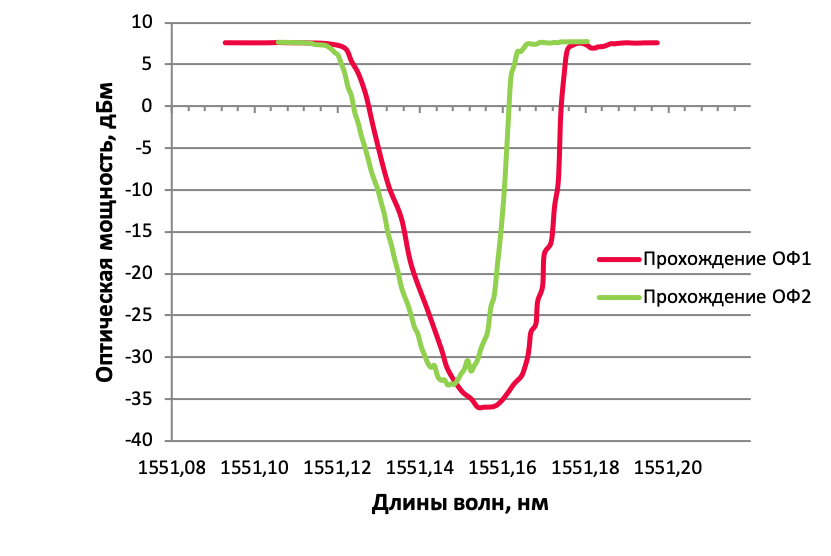
\includegraphics[scale=0.8]{T-spectrums.png}
  \caption{Спектральные характеристики оптических фильтров}
  \label{fig:Spectrums}
\end{figure}

\pagebreak

%%%%%%%%%%%%%%%%%%%%%%%%%%%%%%%%%%%%%%%%%%%%%%%%%%%%%%%%%%%%%%%%%%%%%%%%%%%%%%%%%%%%%%%%%%%%%%%%%%%%%%%%%%%%%%%%%
\section{Экспериментальный стенд} \label{ch:ch5/sect3}

 \begin{figure}[ht]
  \centering
	 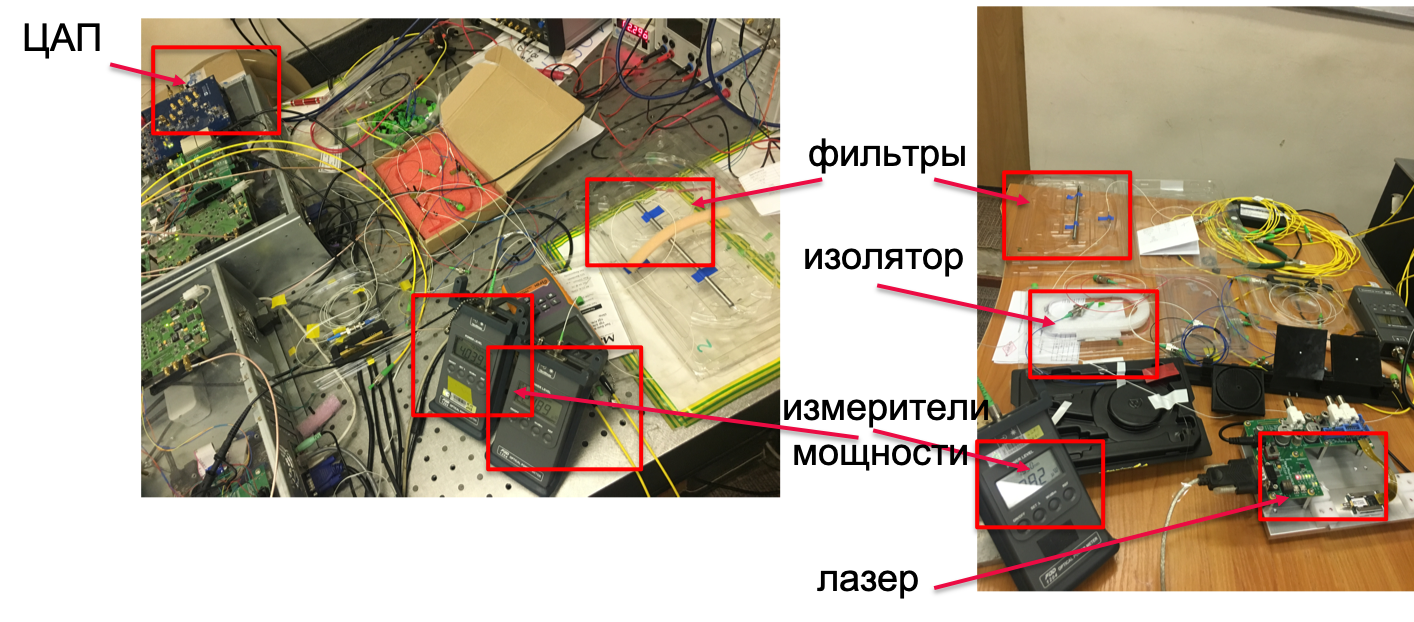
\includegraphics[scale=0.7]{Experimental_setup_TF}
  \caption{Фотография экспериментального стенда}
  \label{fig:experimental_setup_TF}
\end{figure}

\pagebreak

%%%%%%%%%%%%%%%%%%%%%%%%%%%%%%%%%%%%%%%%%%%%%%%%%%%%%%%%%%%%%%%%%%%%%%%%%%%%%%%%%%%%%%%%%%%%%%%%%%%%%%%%%%%%%%%%%
\section{Зависимость интенсивности на боковых частотах от сдвига фаз в результате интерференции в классическом режиме} \label{ch:ch5/sect4}

 \begin{figure}[ht]
  \centering
  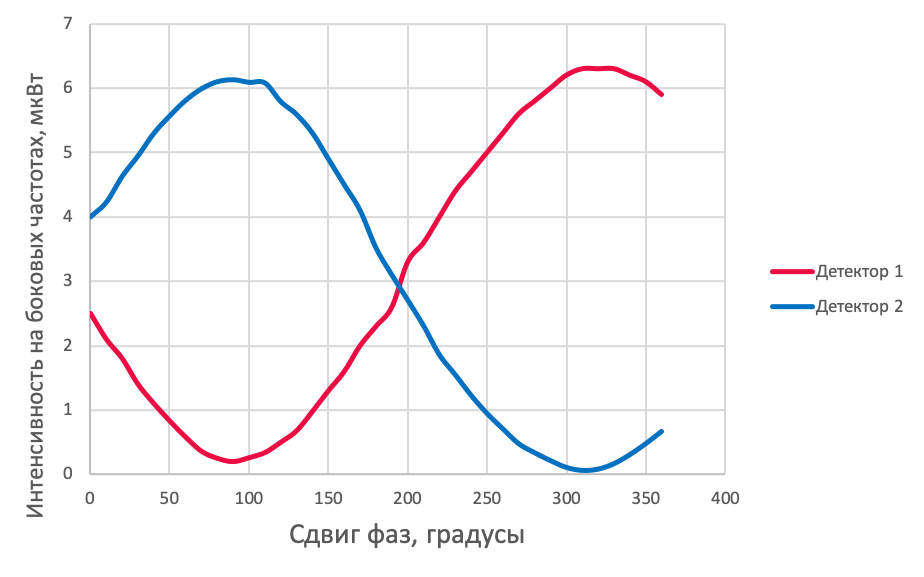
\includegraphics[scale=0.7]{Experimental_TF_classical.png}
  \caption{Зависимость интенсивности на боковых частотах в результате интерференции от разности фаз модулирующих сигналов}
  \label{fig:Experimental_TF_classical}
\end{figure}

\pagebreak

%%%%%%%%%%%%%%%%%%%%%%%%%%%%%%%%%%%%%%%%%%%%%%%%%%%%%%%%%%%%%%%%%%%%%%%%%%%%%%%%%%




\section{Вероятности срабатываний детекторов} \label{ch:ch5/sect5}

 Spectral filter located after beam splitter reflects central optical mode ($k=0$). Hence mean photon number at the entrance of the detector may be found as
\begin{align}\label{nph1}
    n(\Delta\varphi)_{1,2}&=\mu_0\eta_c\Bigg(\sum_{k\neq 0}|d_{0k}^{S}(\beta)|^2 + \vartheta|d_{0k}^{S}(\beta)|^2 \pm \nonumber \\
    &\pm \cos(\varphi_0)\Big(\sum_{k\neq 0}|d_{0k}^{S}(\beta)|^2e^{i\Delta\varphi k}+ \vartheta|d_{0k}^{S}(\beta)|^2 \Big) \Bigg),
\end{align}
where $\Delta\varphi=\varphi_B-\varphi_A$, $\varphi_0$ is relative optical phase between pulses of Alice and Bob, $\vartheta \ll 1$ is part of central mode ($k=0$) due to imperfect spectral filtering. Using the properties of d-function in \cite{varshalovich1988quantum} we simplify previous expression as follows
\begin{align}
    n(\Delta\varphi)_{1,2}=\mu_0\eta_c\Big(1-(1-\vartheta)(1\mp\cos(\varphi_0))|d_{00}^{S}(\beta)|^2 \pm \nonumber \\
    \pm\cos(\varphi_0)d_{00}^{S}(\beta')\Big) \label{nph},
\end{align}
where argument $\beta'$ is as follows
\begin{equation} \label{betaappox}
    \cos(\beta')=\cos^2(\beta) \mp \sin^2(\beta)\cos(\Delta\varphi).
\end{equation}
In order to estimate detection probability we use linear Mandel approximation considering small intensities ($n(\Delta\varphi)_{1,2} \ll 1$):
\begin{eqnarray}
    \mathcal{P}_{1,2}^{+}(\Delta\varphi)=\left(n(\Delta\varphi)_{1,2}\eta_DF+\gamma_{dark}\right)\Delta t, \label{pdet}
\end{eqnarray}
where $\eta_D$ is quantum efficiency, $F$ is frequency of phase changing, $\gamma_{dark}$ is frequency of detector's dark counts, and $\Delta t$ is gating time of the detector. Further we choose $\Delta t F=1$ for simplicity. Absence of detection event we denote as $\mathcal{P}_{1,2}^{-}(\Delta\varphi)=1-\mathcal{P}_{1,2}^{+}(\Delta\varphi)$.     



We introduce useful approximations that help us estimate quantum bit error rate (QBER) and sifted key rate. First of all we consider the case of large number of interaction modes ($S\rightarrow \infty$) which is true for standard optical fiber modulators. One may use approximation of d-function as follows:
\begin{align}
d_{nk}^S(\beta) &\xrightarrow{S\rightarrow \infty} J_{n-k}(m), \label{limdj} \\
\beta &\propto m, \label{propto}
\end{align}
where $J_k(m)$ is Bessel function of the first kind. Considering small $m$, which is also the case, and recalling classical modulation theory we use first order series approximation of Bessel function.
Also according to Eq.~\ref{betam} $\beta \rightarrow 0$ hence one may use first order series approximations to express Eq.~\ref{betaappox} in terms of $m$ implying proportionality in Eq.~\ref{propto}.
Finally we derive Eq.~\ref{pdet} as follows:
\begin{align}\label{pdet1}
 \mathcal{P}_{1,2}^{+}(\Delta\varphi)&=\mu\eta\Big(1\pm\cos(\Delta\varphi)\cos(\varphi_0)\Big)+ \nonumber
 \\
 &+\vartheta\Big(\mu_c\eta(1\pm\cos(\varphi_0))\Big)+p_{dark},
\end{align}


where $\eta$ is total optical transmission including quantum efficiency, $p_{dark}=\gamma_{dark}\Delta t$ is probability of dark count in time interval $\Delta t$, and $\mu$ and $\mu_c$ are the mean number of photons at the sidebands and at the central mode respectively right after the modulation defined as follows
\begin{align}
    \mu&=\mu_0\sum_{k\neq 0}|d_{0k}^{S}(\beta)|^2, \\
    \mu_c&=\mu_0-\mu=\mu_0(1-\sum_{k\neq 0}|d_{0k}^{S}(\beta)|^2).
\end{align}
Expression in Eq.~\ref{pdet1} gives us explicit relations to experimental parameters and demonstrates how they impact detection probabilities.



\pagebreak

%%%%%%%%%%%%%%%%%%%%%%%%%%%%%%%%%%%%%%%%%%%%%%%%%%%%%%%%%%%%%%%%%%%%%%%%%%%%%%%%%%
\section{Зависимость интенсивности на боковых частотах от сдвига фаз в результате интерференции в режиме счета фотонов} \label{ch:ch5/sect6}


 \begin{figure}[ht]
  \centering
  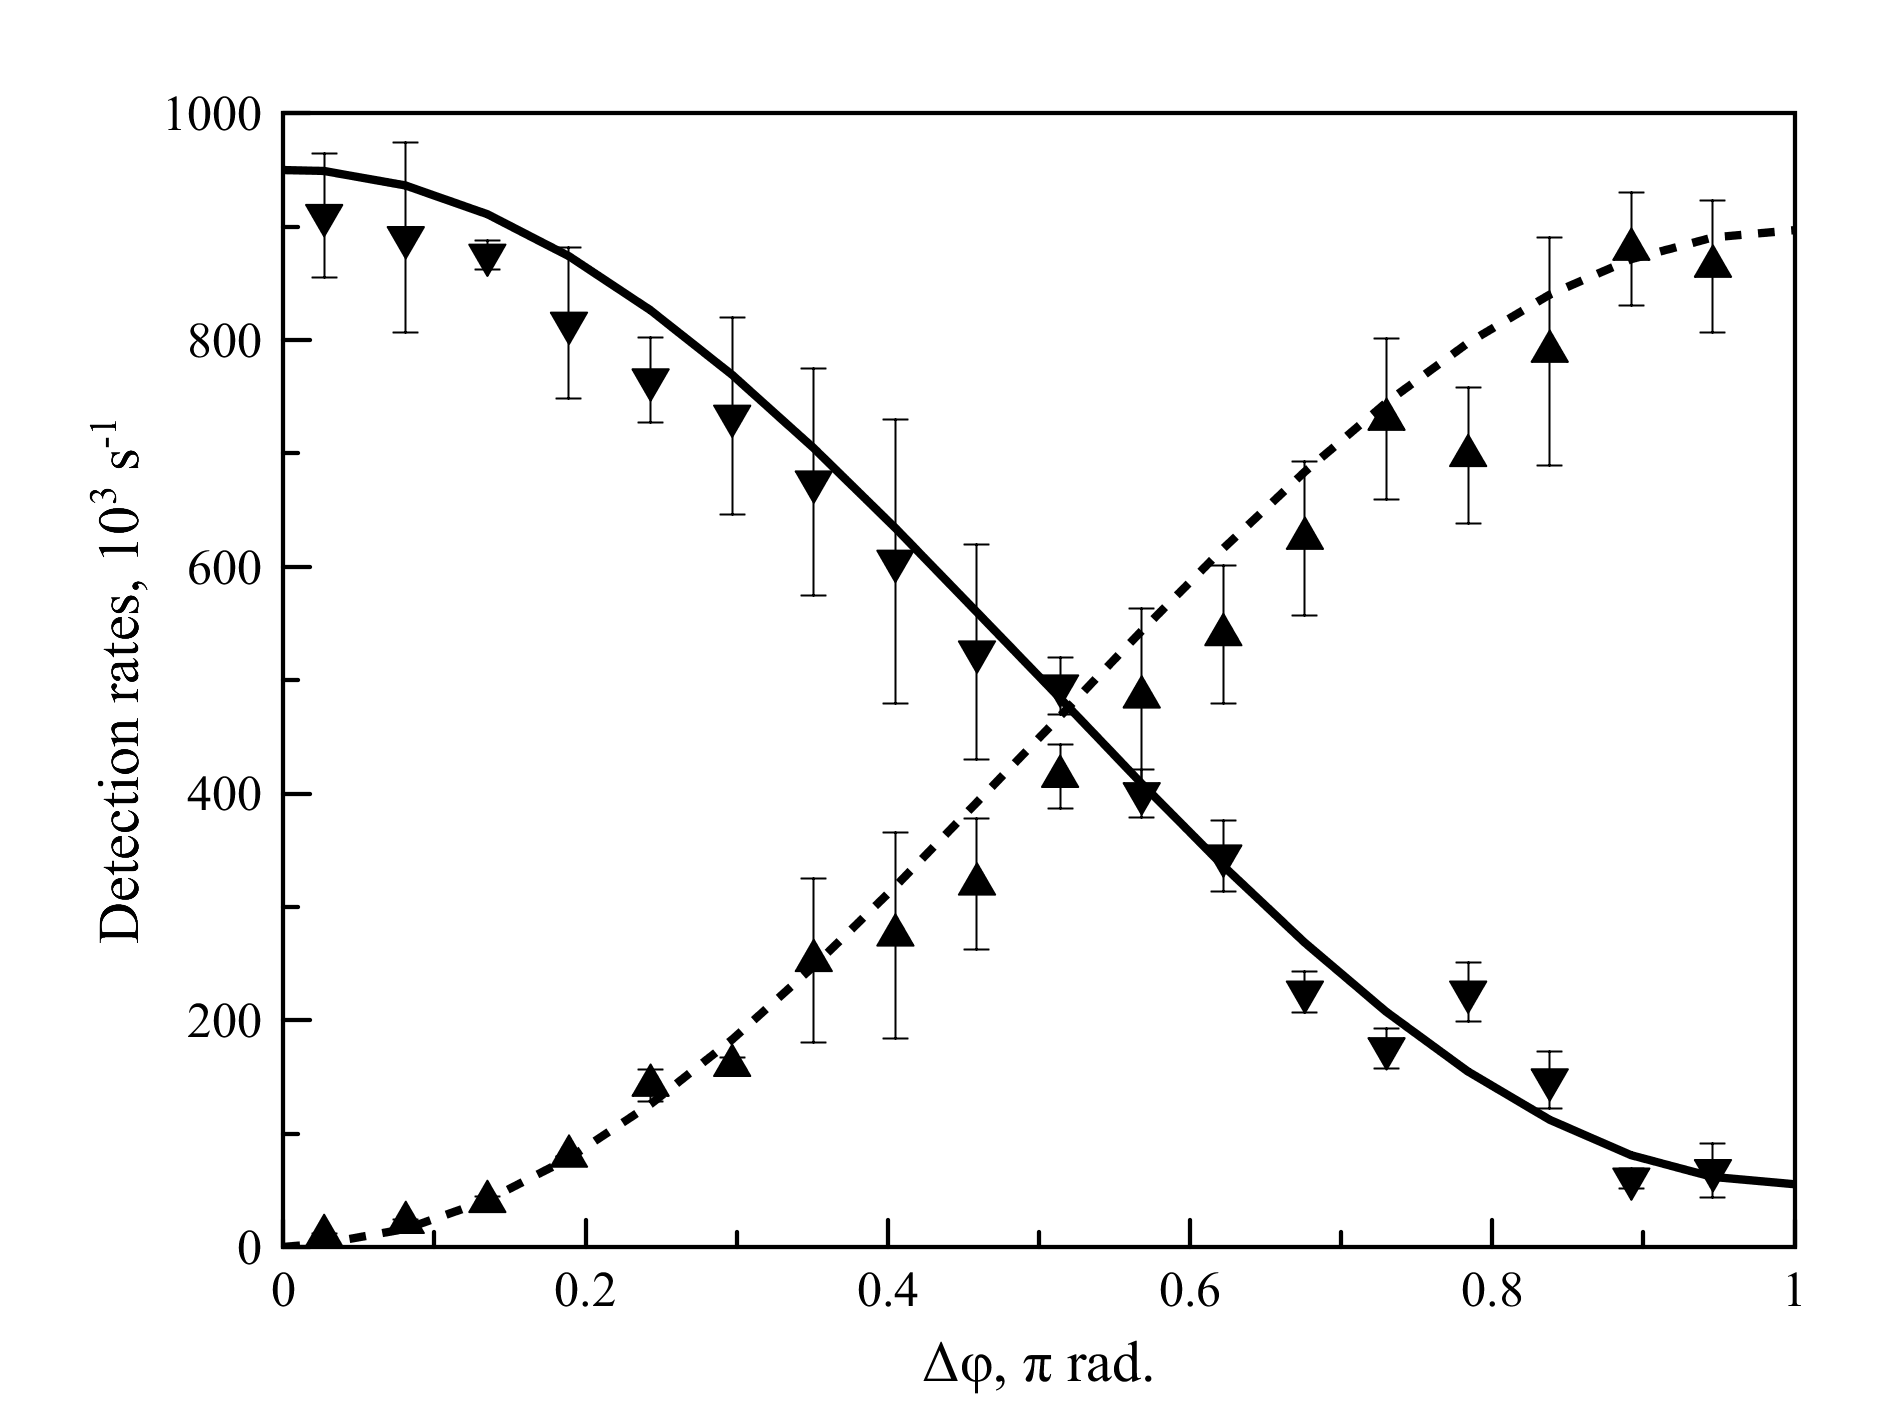
\includegraphics[scale=0.25]{ExperimentTF.png}
  \caption{Зависимость количества отсчетов в результате интерференции от разности фаз модулирующих сигналов}
  \label{fig:Experimental_TF}
\end{figure}


\pagebreak

%%%%%%%%%%%%%%%%%%%%%%%%%%%%%%%%%%%%%%%%%%%%%%%%%%%%%%%%%%%%%%%%%%%%%%%%%%%%%%%%%%
\section{Оценка коэффициента битовых ошибок и скорости формирования ключа} \label{ch:ch5/sect7}

Further we consider only cases where only one of detectors fires. Thus the detection probabilities $R$ is denoted as
\begin{align}
    R&=\Big(\mathcal{P}_{1}^{+}\mathcal{P}_{2}^{-}(\Delta\varphi=\varphi_m)+\mathcal{P}_{1}^{-}\mathcal{P}_{2}^{+}(\Delta\varphi=\pi+\varphi_m)+ \nonumber \\
    &+\mathcal{P}_{1}^{+}\mathcal{P}_{2}^{-}(\Delta\varphi=\pi+\varphi_m)+\mathcal{P}_{1}^{-}\mathcal{P}_{2}^{+}(\Delta\varphi=\varphi_m)\Big),
\end{align}



where $\varphi_m$ is mean phase-mismatch between phases $\varphi_A$ and $\varphi_B$. The first two summand are probabilities of successful bit identification by legitimate users while the second two summands are probabilities of bitflip (assuming $\varphi_0 \approx 0$). Thus one may derive expression for QBER $Q$ as follows
\begin{align}
    Q=\frac{\mathcal{P}_{1}^{-}\mathcal{P}_{2}^{+}(\Delta\varphi=\varphi_m)+\mathcal{P}_{1}^{+}\mathcal{P}_{2}^{-}(\Delta\varphi=\pi+\varphi_m)}{R}.
\end{align}
Finally one may derive expression that estimates average sifted key rates $K$ (identical bits but correlated with Eve hence privacy amplification is necessary)
\begin{equation}
    K=FR(1-h(Q)),
\end{equation}
where $h(Q)$ is binary entropy function.
\pagebreak

%%%%%%%%%%%%%%%%%%%%%%%%%%%%%%%%%%%%%%%%%%%%%%%%%%%%%%%%%%%%%%%%%%%%%%%%%%%%%%%%%%
\section{Выводы по главе} \label{ch:ch5/sect5}


В \ref{ch:ch5} главе показано, что в результате интерференции квантового фазомодулированного сигнала на боковых частотах на симметричном светоделителе в схеме квантовой рассылки ключа с узлом регистрации, независящим от легитимного пользователя, происходит спектральное разделение квантового сигнала и сигнала на центральной длине волны с их независимой регистрацией в разных плечах светоделителя. 

\pagebreak
